\scanpage{84}

fixing the arguments $t_j$ for $j\ne i$, $L_k(t)=L_k(t_1,-t_n)$ \deleted{\unsure{becomes|would be} \deleted{\illegible{1}} a strictly decreasing linear function \deleted{\unsure{it|$t_i$}} of $s=t_i$, bounded above by the continuous increasing function $\inserted{\varphi(\unsure{s|t})=}\varphi(t_1,-t_n)$, \deleted{\unsure{therefore}} which is manifestly impossible, \deleted{\unsure{since}}}\newline
\deleted{for $\unsure{\lambda_i|\lambda}$}\newline
\deleted{$\lambda(s)\to+\infty$ if $s\to-\infty$, and that $\varphi(s)$ remains bounded as $s\to-\infty$.}

one would have $L(t)\to0$ if $t_i\to-\infty$, whereas $\varphi(t)$ \deleted{\unsure{remaining|would remain}}\inserted{would remain} bounded as $t_i\to-\infty$, which \deleted{(\illegible{1} $\unsure{\varphi(t)}$} is incompatible with $L(t)\leq\varphi(t)$ for \deleted{every} $t$. \deleted{\unsure{$f$}} Since \deleted{\unsure{now}}\inserted{finally} $\varphi$ is also assumed symmetric, $L\deleted{\unsure{(t_1,-t_n)}}\leq\varphi\deleted{\unsure{(t_1,-t_n)}}$ \inserted{($L$ a function on $R^n$)} implies $\deleted{\unsure{L_k(t_{\sigma1},-t_{\sigma n})\leq\varphi(t_{\sigma1},\mathord{-}\,\mathord{-}t_{\sigma n})}}\inserted{\sigma L\leq\varphi}$ for \deleted{every} $\sigma\in\mathscr S_n$ (group of permutations of the first $n$ integers, i.e. \inserted{with $\sigma L(t_1,-t_n)=L(t_{\sigma^{-1}1},\mathord{\cdot}\,\mathord{-}t_{\sigma^{-1}n})$}), hence one will also have

\[
\begin{array}{ll}
(7)&\displaystyle\deleted{\unsure{\varphi(t_1,-t_n)|\varphi(t)}}\varphi=\operatorname*{Sup}_k\operatorname*{Sup}_{\sigma\in\mathscr S_n}\sigma.L_k\deleted{\unsure{(t_1,-,t_n)}}
\end{array}
\]

It follows that \deleted{\unsure{if}} to prove (1), it suffices to prove that \inserted{for $L\unsure{\in|=}L_k$, one has} \deleted{$\sigma L_k\deleted{\unsure{(\alpha_{\sigma1})}}\inserted{(\alpha_1,-\alpha_n)}\leq\varphi(\beta_1,-\beta_n)$ for \deleted{every} $k$, and every $\sigma\in\mathscr S_n$. \unsure{Replacing|Let us replace} \inserted{\deleted{\unsure{Denoting|Let us denote}}} $L=$ $\sigma L_k$ by $L$, one is reduced to proving}

\[
\begin{array}{ll}
(8)&\displaystyle\operatorname*{Sup}_{\sigma\in\mathscr S_n}(\sigma.L)(\alpha_1,\mathord{-}\,\mathord{\cdot}\alpha_n)\leq\operatorname*{Sup}_{\sigma\in\mathscr S_n}(\sigma L)(\beta_{\sigma1},\mathord{-}\,\mathord{-}\beta_{\unsure{\sigma n}})
\end{array}
\]

(for the second member is indeed $\leq\varphi(\beta_1,-\beta_n)$)\newline
\reversemarginpar\margin{\begin{tikzpicture}[x=1cm,y=1cm]\draw[red,line width=.4pt] (0,0)--(.02,.35);\end{tikzpicture}}\normalmarginpar
\begin{tikzpicture}[overlay,x=1cm,y=1cm]\draw[red,line width=.35pt] (0,-.22) .. controls (.45,-.38) and (.80,-.36) .. (1.25,-.28) .. controls (1.80,-.18) and (2.35,-.30) .. (2.90,-.29) .. controls (3.40,-.34) and (3.85,-.30) .. (4.20,-.24);\end{tikzpicture}
\deleted{\unsure{For the|In}}\inserted{In this} inequality, \deleted{\unsure{$L$ is a linear form}} \inserted{$L(t_1,-t_n)=\sum_i^n a_it_i+b$}, \deleted{\unsure{affine and}} with \deleted{\unsure{$a_i$}} arbitrary coefficients for in case b), and $a_i>0$ for every $i$ in case a) of the lemma. \deleted{\inserted{\unsure{Let us denote}} \unsure{Let us note},} \inserted{One can obviously} \deleted{\unsure{elementary result} \unsure{well} \illegible{1} \inserted{\unsure{It suffices to prove that}}} suppose $b=0$.

\deleted{By a known lemma, It suffices \deleted{$\sum a_i\unsure{b_i}$} $L(\alpha_1,-,\alpha_n)\leq L(\quad$ \unsure{Let us note that} $\sum a_i\alpha_i\leq\sum a_i\alpha_{\sigma i}$ when $\sigma$ is a permutation such that the sequence of the $a_{\sigma i}$ is \uline{decreasing}, which}

By a known lemma, \inserted{valid \unsure{therefore since|because of the fact that} $\alpha_1\geq\alpha_2\geq-\geq\alpha_n$,} the sum $\sum a_{\sigma i}\alpha_i\inserted{=\sum a_i\alpha_{\sigma^{-1}i}}$ is a maximum, for $\sigma\in\mathscr S_n$ variable,

\reversemarginpar\margin{85}\normalmarginpar
